\documentclass[tikz]{standalone}

\usetikzlibrary{arrows,shadows,positioning,fit,bending}

\begin{document}

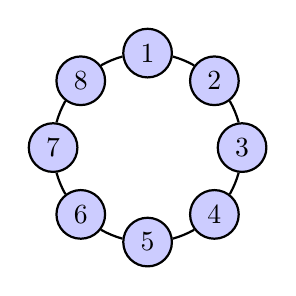
\begin{tikzpicture}[
        thick,
        main node/.style={circle, fill=blue!20, draw, align=center},
    ]
    \newcommand*{\MainRadius}{1.2cm}
    \newcommand*{\MainStartAngle}{90}

    \coordinate (M) at (0, 0);

    \newcommand*{\MainAngleSum}{0}
    \begin{scope}
        % First the nodes are only set, but clipped to get their size.
        % The final location is not yet known.
        \clip (M);
        \foreach \t [count=\i] in {1, 8, 7, 6, 5, 4, 3, 2} {
                \global\expandafter\let\csname p\i-text\endcsname\t
                \node[main node] (p\i) at (M) {\t};
                %
                \global\let\MainNum\i % the last assignment is number of nodes
                % Calculate the angle between the equal sides of the triangle
                % with side length \MainRadius, \MainRadius and radius of circle node
                % Result is stored in \p1-angle, \p2-angle, ...
                \pgfextracty{\dimen0 }{\pgfpointanchor{p\i}{north}}
                \pgfextracty{\dimen2 }{\pgfpointanchor{p\i}{center}}
                \dimen0=\dimexpr\dimen2 - \dimen0\relax
                \ifdim\dimen0<0pt \dimen0 = -\dimen0 \fi
                \pgfmathparse{2*asin(\the\dimen0/\MainRadius/2)}
                \global\expandafter\let\csname p\i-angle\endcsname\pgfmathresult
                \pgfmathparse{\MainAngleSum + 2*\csname p\i-angle\endcsname}
                \global\let\MainAngleSum\pgfmathresult
            }
    \end{scope}
    \pgfmathsetmacro\MainAngleStep{(360 - \MainAngleSum)/\MainNum}

    % Draw the nodes and arrow arcs
    \global\let\CurrentAngle\MainStartAngle
    \foreach \i in {1, ..., \MainNum} {
            \pgfmathsetmacro\AngleA{\CurrentAngle + \csname p\i-angle\endcsname}
            \pgfmathsetmacro\AngleB{\AngleA + \MainAngleStep}
            \draw
            (M) +(\CurrentAngle:\MainRadius)
            node[main node] {\csname p\i-text\endcsname}
            +(\AngleA:\MainRadius)
            arc[
                    start angle=\AngleA,
                    end angle=\AngleB,
                    radius=\MainRadius,
                ]
            ;
            \ifnum\i<\MainNum
                \pgfmathparse{
                    \AngleB
                    + \csname p\the\numexpr\i+1\relax-angle\endcsname
                }
                \global\let\CurrentAngle\pgfmathresult
            \fi
        }
\end{tikzpicture}

\end{document}